
\documentclass[11pt]{article}
\usepackage[a4paper,margin=1in]{geometry}
\usepackage[T1]{fontenc}
\usepackage[utf8]{inputenc}
\usepackage{lmodern,microtype}
\usepackage{amsmath,amssymb,amsthm,mathtools}
\usepackage{graphicx,booktabs,float,enumitem}
\usepackage{xcolor}
\usepackage[colorlinks=true,linkcolor=blue!55!black,citecolor=blue!55!black,urlcolor=blue!55!black]{hyperref}
\usepackage[nameinlink,capitalise,noabbrev]{cleveref}

\newtheorem{theorem}{Theorem}[section]
\newtheorem{proposition}[theorem]{Proposition}
\newtheorem{corollary}[theorem]{Corollary}
\theoremstyle{definition}
\newtheorem{definition}[theorem]{Definition}
\newtheorem{remark}[theorem]{Remark}
\newtheorem{example}[theorem]{Example}

\newcommand{\C}{\mathbb C}
\newcommand{\E}{\mathcal E}
\newcommand{\Oterm}{\mathcal O}

\title{Variational Geometry of Optimal Pandrosion Charts\\
\large Curvature Energies, Euler Directions, and Finite-Dimensional Chart Descent}
\author{Ivan Besevic\\Independent Mathematical Research\\\texttt{github.com/ivan-fr/poussiere\_de\_x}}
\date{May 2026}

\begin{document}
\maketitle

\begin{abstract}
Anchored divided-difference iteration has a local multiplier controlled by the logarithmic curvature of the transformed equation $F_\phi=G\circ\phi$. Earlier chart optimization cancels the pointwise quadratic defect $F''_\phi(r)=0$, and higher-order inverse jets flatten $G\circ\phi$ to arbitrary finite order. This paper proposes a variational continuation: instead of canceling only a finite jet at one root, choose charts by minimizing a curvature energy
\[
\E(\phi)=\int_D \left|\frac{F_\phi''(s)}{F_\phi'(s)}\right|^2w(s)\,ds.
\]
The integrand is the square of the charted logarithmic curvature
\[
\kappa_\phi=(\log F_\phi')'
=\frac{G''(\phi)}{G'(\phi)}\phi'+\frac{\phi''}{\phi'}.
\]
Local curvature cancellation is the pointwise condition $\kappa_\phi(r)=0$, while the exact inverse chart makes $\kappa_\phi\equiv0$. In constrained chart families, such as polynomial jets, variational minimization gives a finite-dimensional normal equation for the best available flattening. Figures for $G(z)=e^z-2$ show the curvature-energy landscape in a quadratic-cubic family, the gradient-descent path toward inverse-jet coefficients, and the decay of energy along higher inverse-jet truncations. The central message is that optimal chart selection can be formulated as a variational geometry of analytic coordinates.
\end{abstract}

\paragraph{One-sentence summary.}
The scalar chart-selection law becomes a variational principle: minimize the $L^2$ energy of the logarithmic curvature $\kappa_\phi=F''_\phi/F'_\phi$.

\section{Introduction}

The anchored divided-difference multiplier near a simple root is
\[
P'_{\phi,a}(r)
=
\frac{F''_\phi(r)}{2F'_\phi(r)}(a-r)+\Oterm((a-r)^2).
\]
Thus the ratio
\[
\kappa_\phi(r)=\frac{F''_\phi(r)}{F'_\phi(r)}
\]
is the local curvature that controls the residual. The optimal-chart paper cancels this curvature at a point. The higher-order jet paper cancels more Taylor coefficients at the same point.

The present paper asks a different question: can chart selection be made variational? Instead of imposing one pointwise constraint, we minimize an energy measuring how nonlinear the transformed equation is over a neighborhood.

\section{The logarithmic curvature of a chart}

Let $G$ be analytic near a simple zero $\rho$, and let $\phi$ be a local chart. Set
\[
F_\phi(s)=G(\phi(s)).
\]
Assume $F_\phi'(s)\neq0$ on a small domain $D$.

\begin{definition}[Chart curvature]
The logarithmic curvature of the charted equation is
\begin{equation}\label{eq:kappa}
\kappa_\phi(s)=\frac{F_\phi''(s)}{F_\phi'(s)}
=(\log F_\phi'(s))'.
\end{equation}
\end{definition}

By the chain rule,
\begin{equation}\label{eq:kappa-transform}
\kappa_\phi(s)
=
\frac{G''(\phi(s))}{G'(\phi(s))}\phi'(s)
+
\frac{\phi''(s)}{\phi'(s)}.
\end{equation}
This is the same expression that appeared in the local chart multiplier law.

\begin{proposition}[Pointwise curvature cancellation]
Let $r$ be the root coordinate. A root-normalized chart satisfies
\[
P'_{\phi,a}(r)=\frac12\kappa_\phi(r)(a-r)+\Oterm((a-r)^2).
\]
Consequently, first-order local optimality is equivalent to
\[
\kappa_\phi(r)=0.
\]
\end{proposition}

\begin{proof}
This is the local multiplier expansion applied to $F_\phi$.
\end{proof}

\section{Curvature energy}

\begin{definition}[Variational chart energy]
Let $D\subset\C$ be a small chart domain and let $w\ge0$ be a weight. Define
\begin{equation}\label{eq:energy}
\E_D(\phi)=\int_D |\kappa_\phi(s)|^2w(s)\,dA(s).
\end{equation}
On a real interval $I$, the corresponding one-dimensional energy is
\[
\E_I(\phi)=\int_I |\kappa_\phi(s)|^2w(s)\,ds.
\]
\end{definition}

This energy vanishes exactly when $F_\phi$ is affine on the domain. If root normalization is imposed, the affine model is $F_\phi(s)=s-r$.

\begin{theorem}[Exact inverse charts are zero-energy minimizers]\label{thm:zero}
Let $G$ be locally invertible near a simple zero $\rho$. If $\phi_*(s)=G^{-1}(s)$ in a neighborhood of $0$, then
\[
G(\phi_*(s))=s,
\qquad
\kappa_{\phi_*}\equiv0,
\qquad
\E(\phi_*)=0.
\]
Conversely, if $\E(\phi)=0$ on a connected domain and $F_\phi'$ is nonzero, then $F_\phi$ is affine. Under root normalization, $F_\phi(s)=s$.
\end{theorem}

\begin{proof}
The inverse chart statement is immediate. Conversely, $\E(\phi)=0$ implies $\kappa_\phi=0$ almost everywhere, hence everywhere by analyticity. Therefore $(\log F_\phi')'=0$, so $F_\phi'$ is constant and $F_\phi$ is affine. Root normalization fixes the affine map to be the identity.
\end{proof}

\section{Finite-dimensional chart families}

In practice one does not optimize over all analytic charts. One chooses a finite-dimensional family
\[
\phi_\theta(s)=\rho+\frac{s}{G'(\rho)}+\sum_{j=2}^m \theta_j s^j.
\]
Then
\[
\E(\theta)=\int_I |\kappa_{\phi_\theta}(s)|^2w(s)\,ds.
\]

\begin{proposition}[Normal equations in a chart family]\label{prop:normal}
Assume $\theta\mapsto\phi_\theta$ is differentiable and $I$ is real. A stationary point of $\E$ satisfies
\begin{equation}\label{eq:normal}
\operatorname{Re}\int_I \overline{\kappa_\theta(s)}
\frac{\partial \kappa_\theta(s)}{\partial \theta_j}
w(s)\,ds=0
\qquad(j=1,\dots,N).
\end{equation}
\end{proposition}

\begin{proof}
Differentiate $\E(\theta)=\int |\kappa_\theta|^2w$ under the integral sign:
\[
\frac{\partial\E}{\partial\theta_j}
=
2\operatorname{Re}\int \overline{\kappa_\theta}
\frac{\partial\kappa_\theta}{\partial\theta_j}w.
\]
Setting the derivative to zero gives \eqref{eq:normal}.
\end{proof}

\begin{remark}
The normal equations are the variational analogue of the jet cancellation equations. Jet cancellation imposes vanishing Taylor coefficients at one point. Energy minimization distributes the flattening over a domain.
\end{remark}

\section{Example: \texorpdfstring{$G(z)=e^z-2$}{G(z)=exp(z)-2}}

Let $\rho=\log 2$ and consider the real chart family
\[
\phi_{\eta,\zeta}(s)=\rho+\frac{s}{2}+\eta s^2+\zeta s^3.
\]
For $G(z)=e^z-2$, one has $G''/G'=1$, so
\[
\kappa_{\eta,\zeta}(s)
=
\phi_{\eta,\zeta}'(s)
+
\frac{\phi_{\eta,\zeta}''(s)}{\phi_{\eta,\zeta}'(s)}.
\]
The exact inverse is
\[
\log(2+s)=\rho+\frac{s}{2}-\frac{s^2}{8}+\frac{s^3}{24}-\cdots.
\]
Thus the quadratic-cubic inverse jet has
\[
\eta_*=-\frac18,\qquad \zeta_*=\frac1{24}.
\]

We use the weighted interval energy
\[
\E(\eta,\zeta)=
\frac{\int_{-0.65}^{0.65}|\kappa_{\eta,\zeta}(s)|^2e^{-(s/0.55)^2}\,ds}
{\int_{-0.65}^{0.65}e^{-(s/0.55)^2}\,ds}.
\]

\begin{figure}[H]
\centering
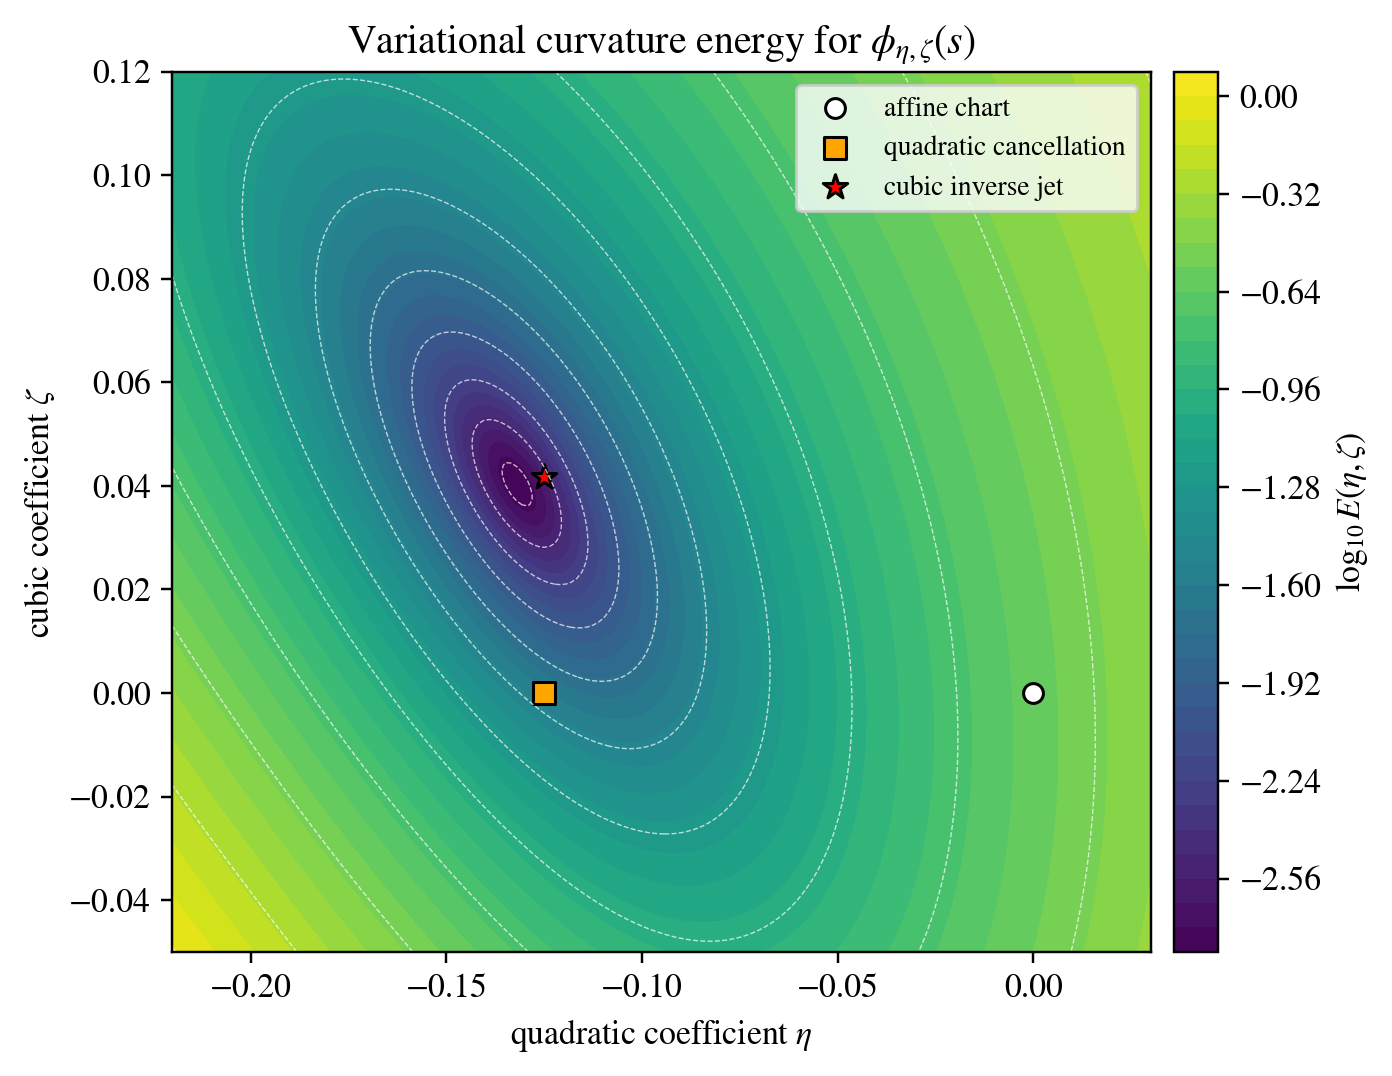
\includegraphics[width=.80\textwidth]{figures/fig_variational_energy_landscape.png}
\caption{Curvature-energy landscape for the quadratic-cubic chart family. The affine chart, quadratic cancellation, and cubic inverse jet are marked. The inverse-jet coefficients lie near the low-energy valley.}
\end{figure}

\begin{figure}[H]
\centering
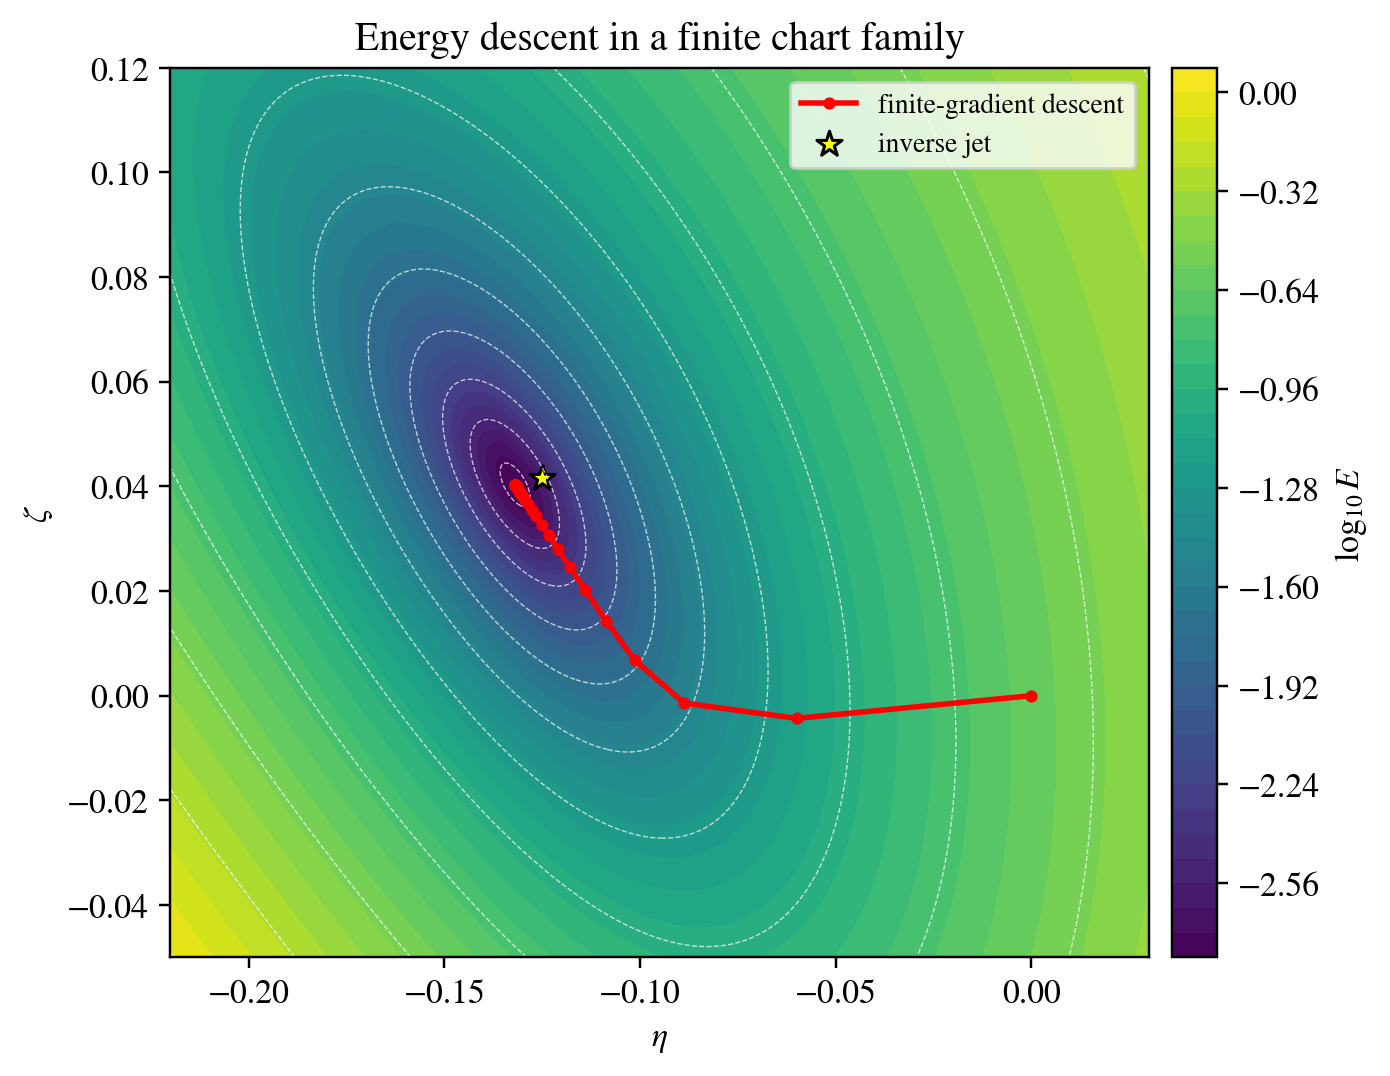
\includegraphics[width=.80\textwidth]{figures/fig_variational_descent_path.png}
\caption{Finite-gradient descent from the affine chart in the same energy landscape. The descent moves toward the inverse-jet valley.}
\end{figure}

\begin{figure}[H]
\centering
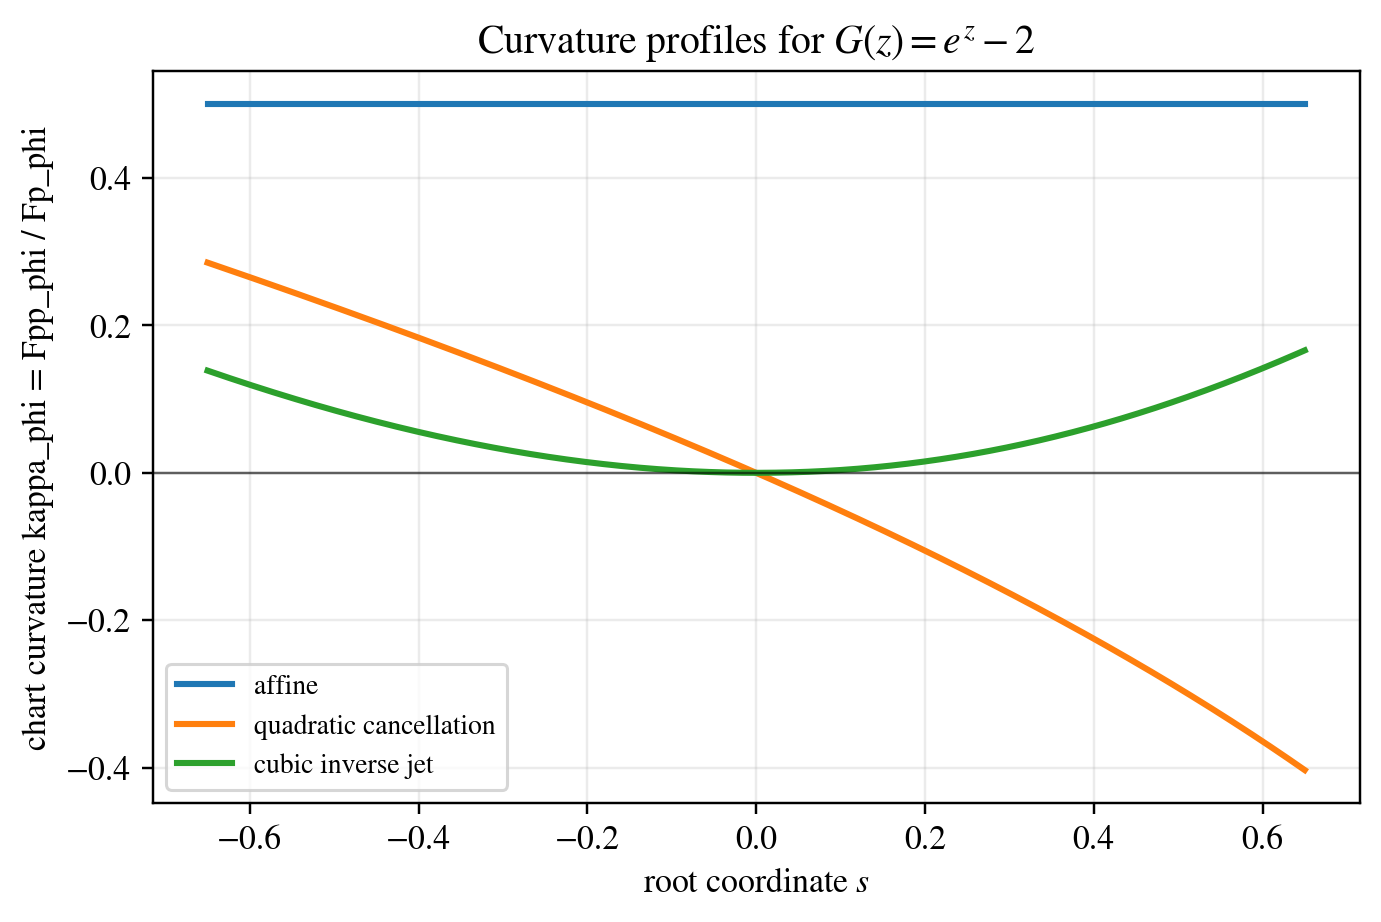
\includegraphics[width=.78\textwidth]{figures/fig_curvature_profiles.png}
\caption{Curvature profiles $\kappa_\phi=F_\phi''/F_\phi'$ on the real root coordinate. The quadratic and cubic inverse-jet charts suppress curvature near the root compared with the affine chart.}
\end{figure}

\begin{figure}[H]
\centering
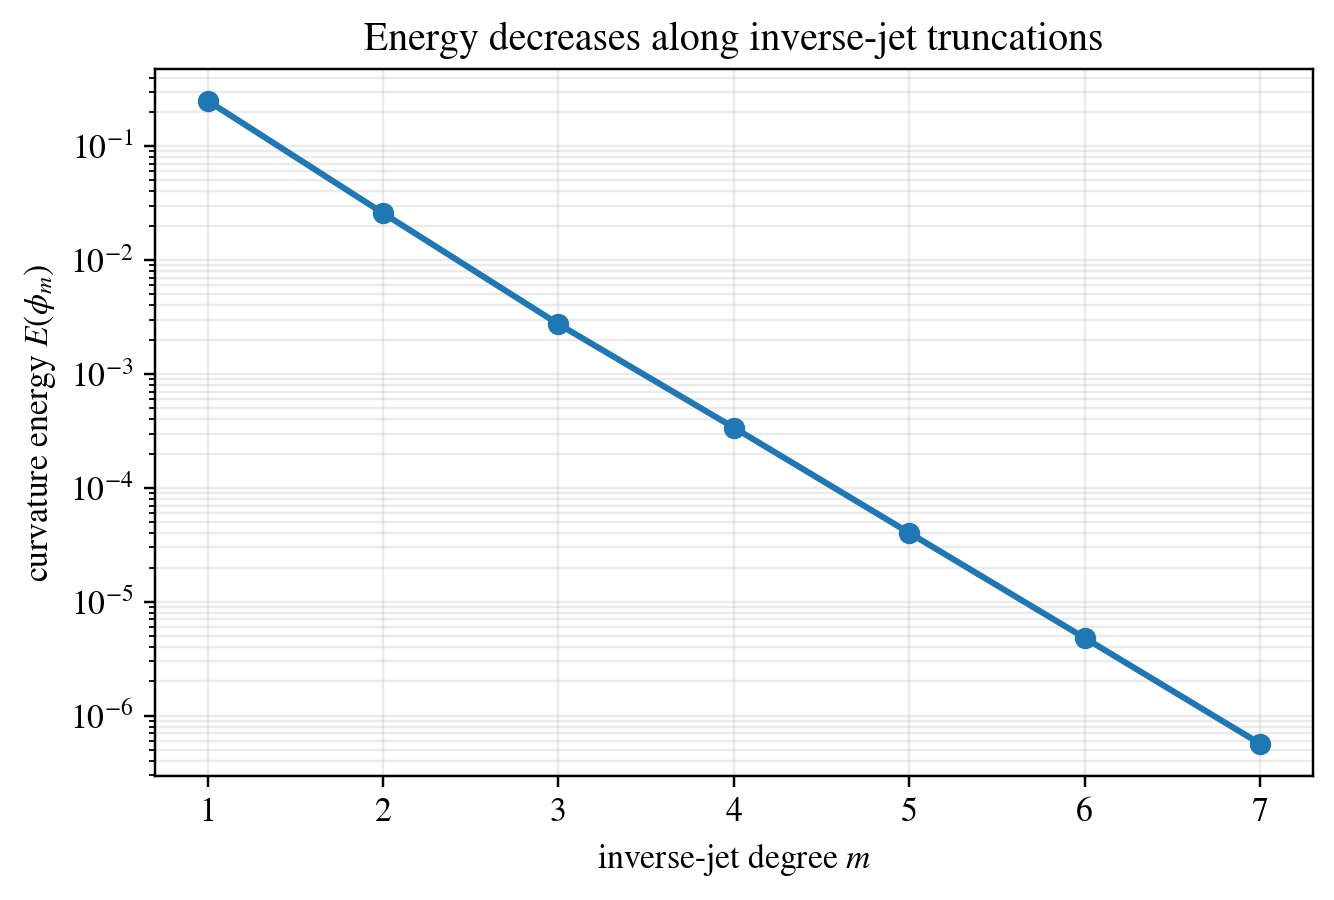
\includegraphics[width=.76\textwidth]{figures/fig_inverse_jet_energy_decay.png}
\caption{Curvature energy along inverse-jet truncations. Increasing the inverse-jet degree reduces the energy over the chosen interval until numerical and truncation effects dominate.}
\end{figure}

\section{Relation with higher-order jet cancellation}

Higher-order jet cancellation is a local normal-form statement:
\[
G(\phi_m(s))=s+\Oterm(s^{m+1}).
\]
Variational chart geometry replaces this pointwise order condition by an integral criterion. The two viewpoints agree in the limit of a shrinking weight. If $w_\epsilon$ concentrates near the root, then minimizing $\E_{w_\epsilon}$ forces successive Taylor coefficients of $\kappa_\phi$ to vanish, recovering inverse-jet cancellation.

\begin{proposition}[Concentration recovers local cancellation]
Let $w_\epsilon(s)=\epsilon^{-1}w(s/\epsilon)$ on a real interval and assume a polynomial chart family contains the inverse jet through degree $m$. As $\epsilon\to0$, any minimizer of $\E_{w_\epsilon}$ whose coefficients remain bounded satisfies the inverse-jet cancellation equations through degree $m$, provided the minimizer is isolated.
\end{proposition}

\begin{proof}
Expanding $\kappa_\phi(s)$ in a Taylor series, the concentrated energy is asymptotically a weighted sum of squared Taylor coefficients with powers of $\epsilon$. The leading nonzero coefficient dominates. Minimization therefore cancels the lowest available coefficient first, then the next, and so on. This is exactly the inverse-jet hierarchy.
\end{proof}

\section{Outlook}

The variational viewpoint suggests several extensions:
\begin{enumerate}[label=(\roman*)]
\item rational chart families, where Padé-type inverse approximants can reduce energy on larger domains;
\item complex-area energies over disks, annuli, or basin neighborhoods;
\item multidimensional tensor energies such as $\int\|D^2(G\circ\phi)\|^2$;
\item adaptive engines that update chart parameters by residual-gated energy descent.
\end{enumerate}

\section{Conclusion}

The local chart-selection law can be globalized into a variational principle. The quantity
\[
\kappa_\phi=\frac{F_\phi''}{F_\phi'}
\]
is both the local multiplier coefficient and the curvature of the transformed equation. Minimizing its energy gives a principled way to choose charts when exact inverse charts are unavailable. This reframes chart selection as a variational geometry of analytic coordinates.

\begin{thebibliography}{9}
\bibitem{monomial}
I. Besevic, \emph{A Monomial Pandrosion Scheme}, manuscript, May 2026.
\bibitem{general}
I. Besevic, \emph{Anchored Pandrosion for General Analytic Equations}, manuscript, May 2026.
\bibitem{charts}
I. Besevic, \emph{Optimal Geometric Charts for Anchored Divided-Difference Iterations}, manuscript, May 2026.
\bibitem{jets}
I. Besevic, \emph{Higher-Order Jet Cancellation for Anchored Divided-Difference Iterations}, manuscript, May 2026.
\bibitem{ahlfors}
L. Ahlfors, \emph{Complex Analysis}, 3rd ed., McGraw--Hill, 1979.
\bibitem{henrici}
P. Henrici, \emph{Applied and Computational Complex Analysis}, Wiley, 1974--1986.
\end{thebibliography}

\end{document}
